\chapter{Remarks about our study}
In this chapter describe in detail the specifications of the simulations we are going to work with. Furthermore, we present the chosen method for determining the halo shapes. This chapter is mainly to thoroughly explain how are we going to do everything that we are going to do.\\

\section{The Auriga simulations}
Cosmological simulations are restricted to modeling DM as a non collisional fluid and gas as an Eulerian(?) collisional fluid. Efficiently solving these systems of non-linear equations is an intricate puzzle and it is still an open and improving field of research. 
Difficulties in the numerical modeling of these fluids arise from the wide range of values that quantities take in the context of cosmological objects, which can expand in several orders of magnitude, are no much different than actual field discontinuities which are very difficult to treat in a numerical way.\\

It is clear that this simulations are limited to some resolution depending on the current power of computing super-clusters. This resolution is variable between simulations and is adjustable to the specific objective of the research. However, this resolution is by no means sufficient to simulate specific termic processes dominated by quantum or particle physics. However, specific details which are consequence of this non-modelable physics, are needed to accurately model cosmological structures. This is why energy and mass feedback processes such as supernovae (SN) explosions, black hole (BH) accretion and radiation, are usually reduced to some simplification dependent on some free parameters. A decade ago, thee feedback processes were not as well understood nor well modeled as they are today. For this reason, and the advances on technology, it has been possible only until recently the simulation of galactic-sized objects like our MW tracking the evolution of normal matter alongside with DM.\\


State all the important specs of the Auriga simulations. On the first paragraph.\\

Talk about the different degrees of realism in this simulation> DM, MHD, resolution levels. State the importance of these aspects for the soundness (look better word) of the studies.\\

\begin{figure}[!ht]
    \centering
    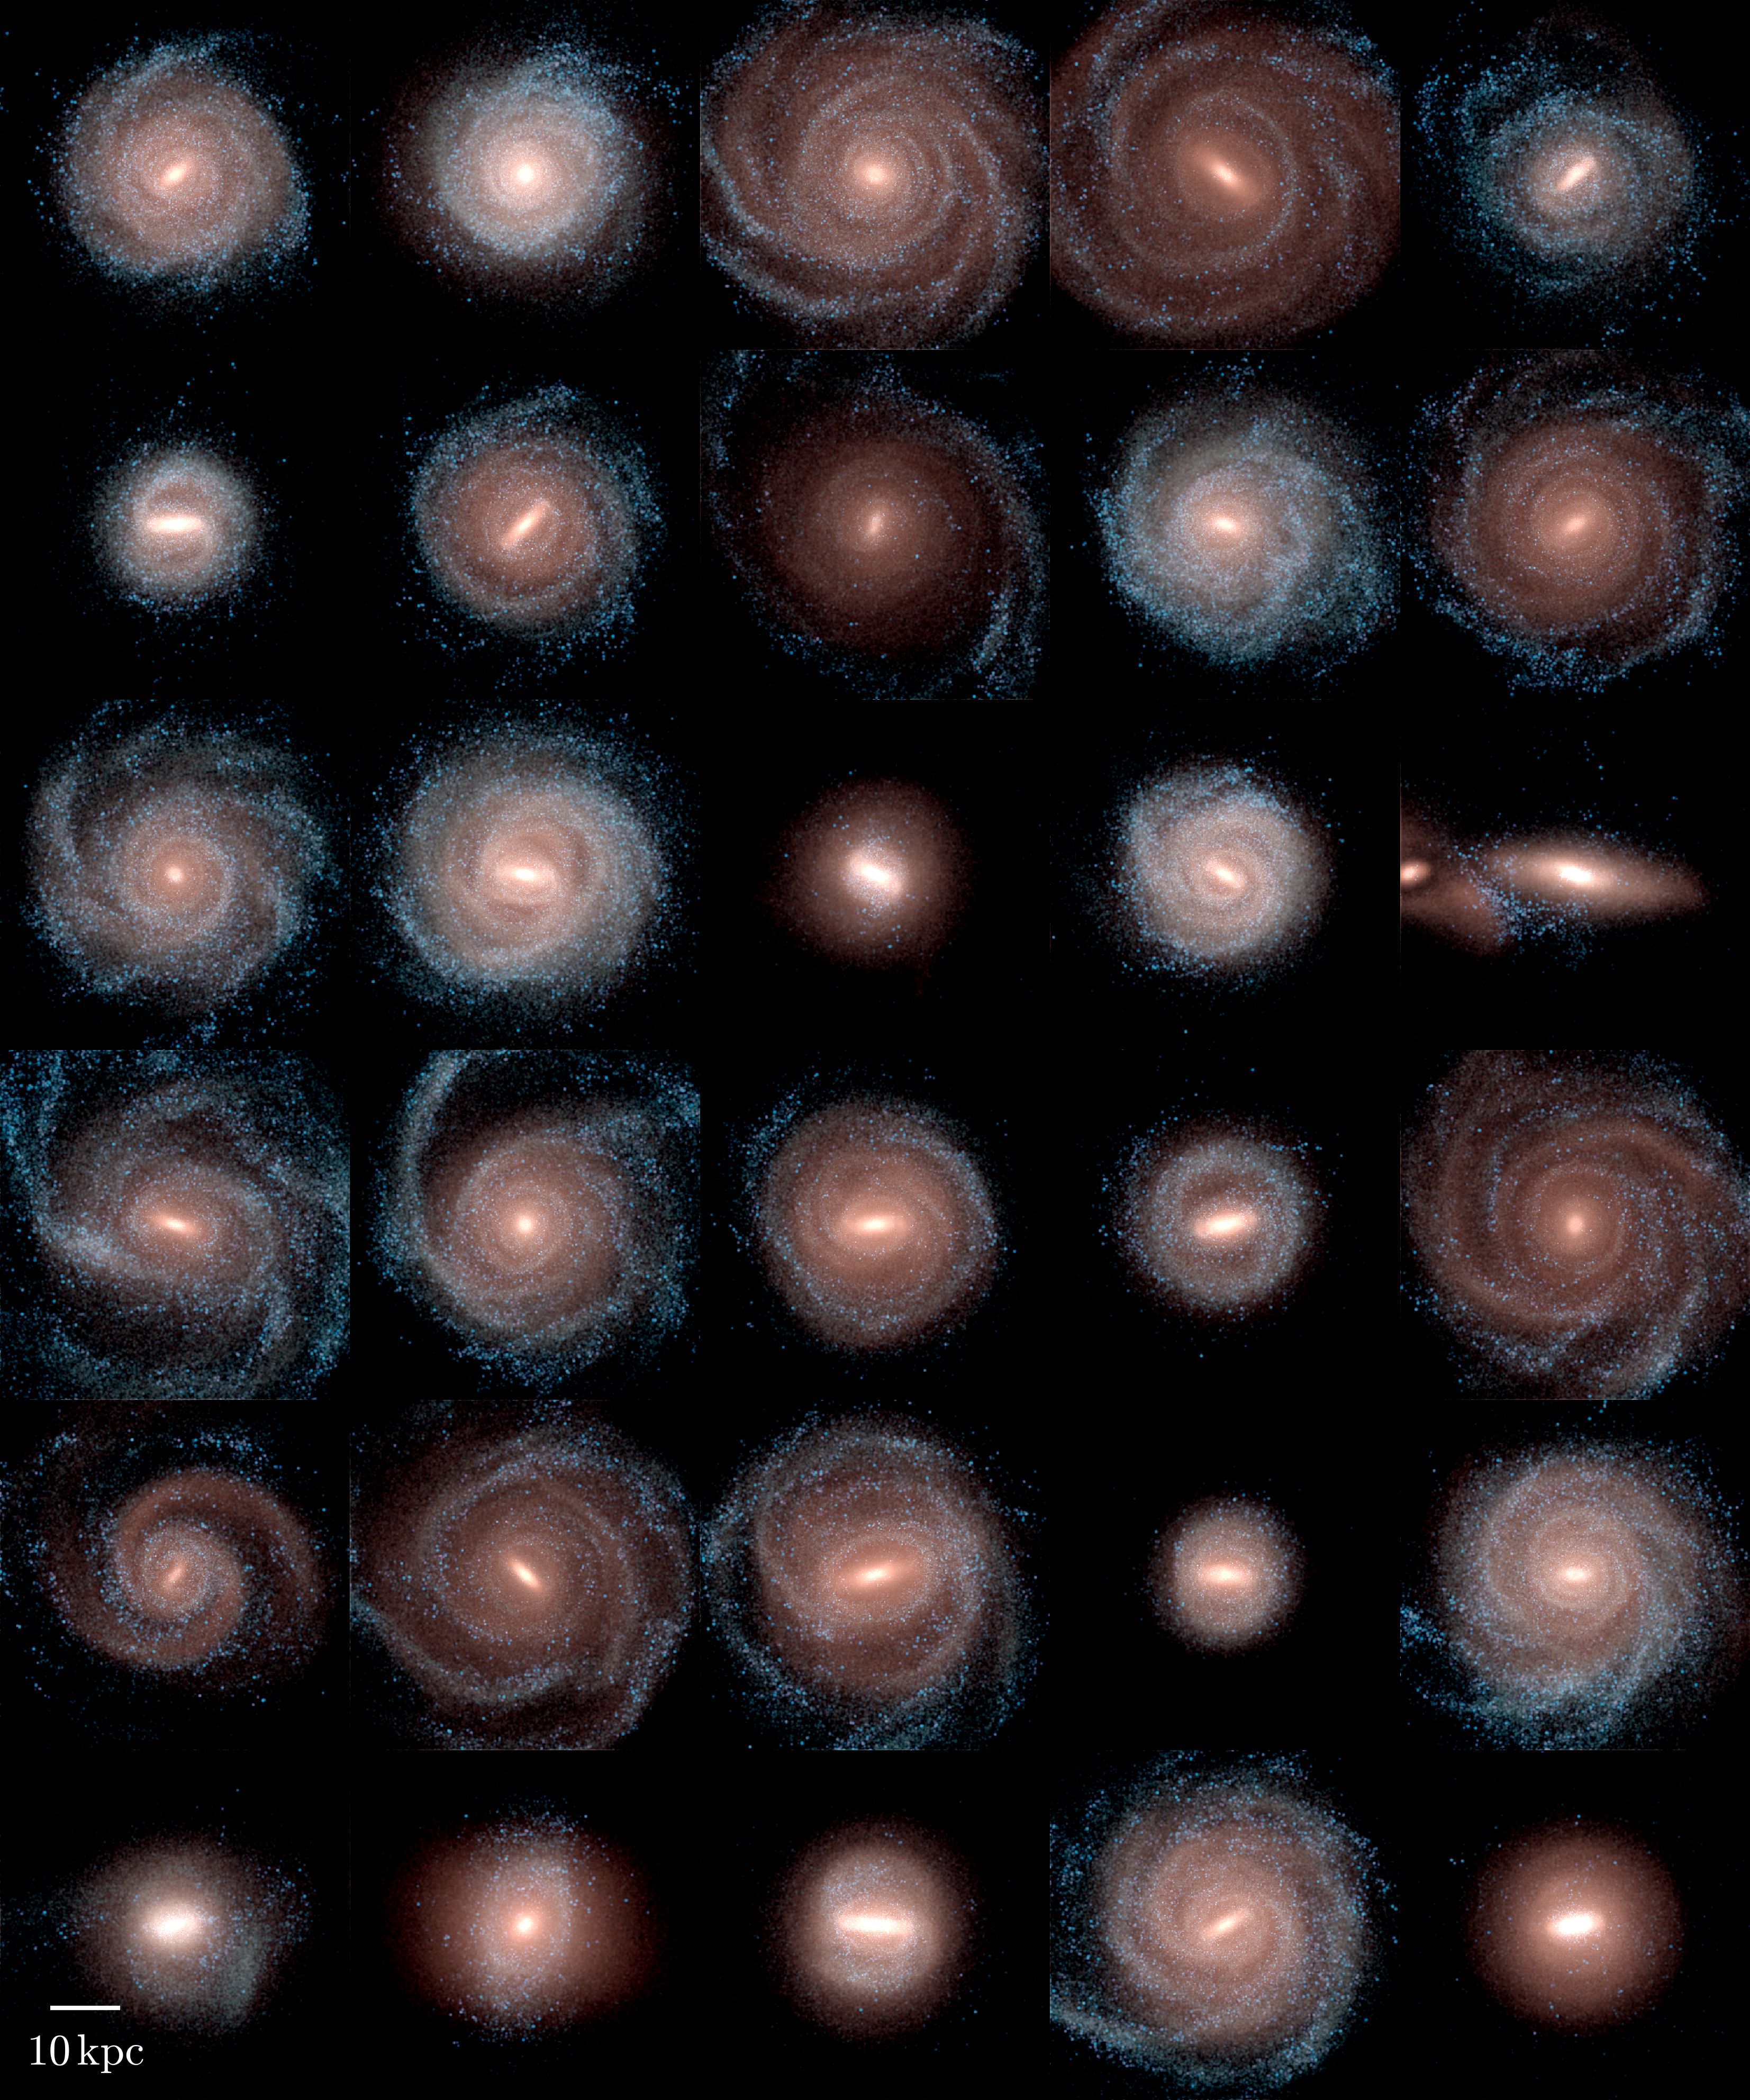
\includegraphics[width=0.8\textwidth]{./pics/Auriga.png}
    \caption{Set of 30 MW-like simulations, taken from http://auriga.h-its.org/}
    \label{fig:auriga}
\end{figure}

\section{Determining the halo shape}
The discretization of the DM density field into particles makes it difficult  to perform some calculations that would require a more continuous distribution such as those related to the density field. The case of the shape of the halo is no exemption, and therefore there is no trivial way to calculate the DM halo shape at a determined radius. There are different approaches to this problem, such as the use of an inertia tensor or the approximation to the respective contour surface.
However, the results do not vary very much from method to method \cite{Vera-Ciro et al. 2011}. In this work we follow the guidelines by Vera-Ciro et al 2011 which includes the use of the shape method by Allgood 2006\cite{AllGood2006}.\\

Allgood's method starts with particles enclosed within a sphere whose radius $r$ is the initial radius where we want to obtain the shape. We calculate the reduced inertia tensor:

\begin{equation}
I_{ij} = \sum_k \frac{x_k^{(i)}x_k^{(j)}}{d^2_k},
\label{eq:inertia}
\end{equation}

which has weighted components by distance $d^2=x^2+y^2+z^2$, so that each particle contribute with same importance to the inertia tensor, neglecting their distance to the center of the halo.\\

The diagonalization of this tensor yields the principal axes of the structure, as well as the eigen-quantities $a>b>c$ which produce the respective axial ratios. However, if we characterize an ellipsoid taking into account only particles enclosed within a sphere, we are effectively underestimating its triaxiality \cite{AllGood}. For this reason, we iteratively recalculate the inertia tensor taking into account the previously characterized ellipsoid.\\

AllGood et al. propose to use the eigenvalues $a>b>c$ and their respective eigen-axes $v_a,v_b,v_c$ to recalculate the inertia tensor over the particles enclosed by the ellipsoid with principal axes (along the respective eigenvectors) equal to $r,r/q,r/s$, where ere $q = b/a$ and $s=c/a$ are the axial ratios. In other words, we repeat the process of calculating the inertia matrix by taking into account particles within an ellipsoid with axial ratios given by the previous diagonalization, maintaining the principal axis of the enclosing ellipsoid constant (this is a freedom choice).\\

This method sounds good and it would eventually converge to a more accurate characterization of the halo ellipsoid. However, we are computing the reduced inertia tensor by weighting the contributions with the spherical-metric distance $d^2=x^2+y^2+z^2$, where particles within the same spherical surface are given the same importance. This means we are again underestimating ??? the triaxiality of the structure. For this reason, on each iteration we must calculate the inertia tensor taking into account an elliptic metric: $\bar{d}^2 = x^2+y^2/q^2+z^2/s^2$, assuming $x,y,z$ are the corresponding principal axes.\\

In case this concept of an elliptic metric is difficult to grasp, let us consider that, instead of converting the initial enclosing sphere to the halo ellipse, we are converting the halo ellipsoid into an sphere by performing scale transforms along the respective eigen-axes. From this point of view, we start our first-guess calculation of the ellipsoid by calculating the reduced inertia tensor \eqref{eq:inertia} for particles enclosed within a sphere of radius $r$. Then with the results of this first guess, we perform the following scale transform:\\
  
\begin{align}
(x,y,z) &\rightarrow (x',y',z')=(x,y/q,z/s) \label{eq:scale}\\
q &=  b/a \nonumber \\
s &= c/a \nonumber ,
\end{align}

where we assumed the axes $x,y,z$ are oriented at the principal axes. We then repeat the process of calculating the reduced inertia tensor and performing the scale transform until we achieve certain convergence criterion. We stop this iterative process when the sum of the fractional change in axes is less than $10^{-6}$ to obtain the shape of the halo at the geometric mean radius $(abc)^{1/3}$, which is not much different from the initial radius.\\

Notice that calculating the inertia tensor with the scaled coordinates $x',y',z'$ is equivalent to calculating it with the un-scaled coordinates $x,y,z$ but using the elliptic-metric distance $\bar{d}^2 = x^2+y^2/q^2+z^2/s^2$, for diagonalization purposes.\\

